% Chapter for alternative methods to solving the problem.

\chapter{Methods}
\label{ch:methods}

In this chapter, we discuss our solution to the problem stated in Chapter
\ref{ch:intro}, as well as various alternatives we considered along the way.
First, we briefly introduce the schematic entry GUI.
Next, we discuss in detail how we solved the automatic protoboard layout
problem and how we evaluated our solution.

\section{GUI}

We designed the schematic entry GUI to have a rich set of features so as to make
drawing schematics an easy and intuitive task for students.
Figure \ref{fig:gui_example} gives a version of the schematic shown in Figure
\ref{fig:schematic} as drawn in the schematic entry tool. Appendix \ref{app:gui}
discusses the features and capabilities of the schematic entry GUI in
further detail.

\begin{figure}
\begin{center}
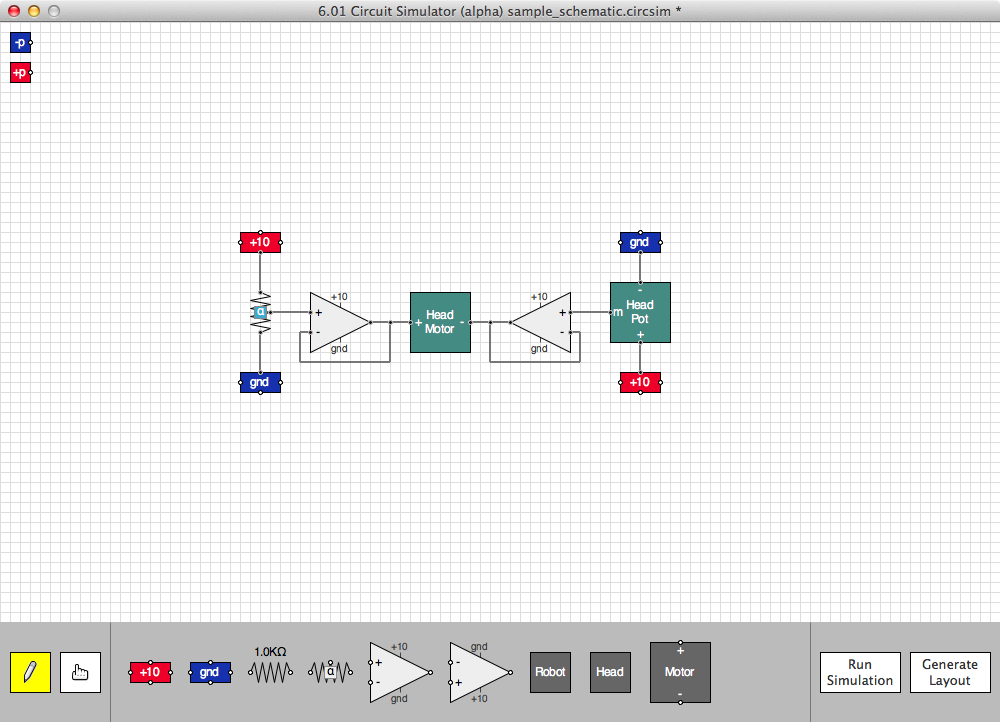
\includegraphics[width=\textwidth]{Images/gui_example.png}
\caption[Schematic entry example]{Sample schematic drawn on the schematic entry
tool. This schematic describes the same circuit as the one described by the
schematic shown in Figure \ref{fig:schematic}.}
\label{fig:gui_example}
\end{center}
\end{figure}

\section{Solving the Layout Problem}

In broad terms, we solved the layout problem by formulating it as a graph search
problem. Given a schematic of a circuit, we start from an empty
protoboard, and search through the space of all possible protoboard layouts to
find a good protoboard layout for the schematic at hand. Importantly, we
utilize various simplifications and heuristics to prune out many states in the
search space.

We broke down the problem into two parts. The first task is finding a placement
of all the circuit pieces on the protoboard. The second task is putting down
wires to appropriately connect the pieces.

\subsection{Part 1: Placement}
\label{sec:placement}

Let us first consider how to place a set of circuit pieces on the protoboard for
a given circuit schematic. Any given circuit may contain resistors, pots,
op-amps, motors, robot parts, or head connector connector parts.
For each of these
components, we must put down a corresponding piece on the protoboard. As each
piece may be placed on the protoboard in one of many different ways, we first
decided on a fixed set of allowed placements for each of the pieces. Figure
\ref{fig:piece_placement} presents these acceptable placements.
Resistors are placed in the middle strip of the protoboard.
Pots have two possible vertical positions as well as two possible orientations.
The connector pieces have two possible vertical positions each.
Op-amp pieces are also placed in the middle strip of the protoboard, but with
two possible orientations. Op-amp pieces are unique in that, as shown in Figure
\ref{fig:op_amp_pin_out}, each op-amp piece
contains two op-amps within it. Thus, we face the task of packaging the op-amps
in the schematic in the ``best'' possible way, i.e. so as to require as little
work as possible when wiring the pieces together.

\begin{figure}
\begin{center}
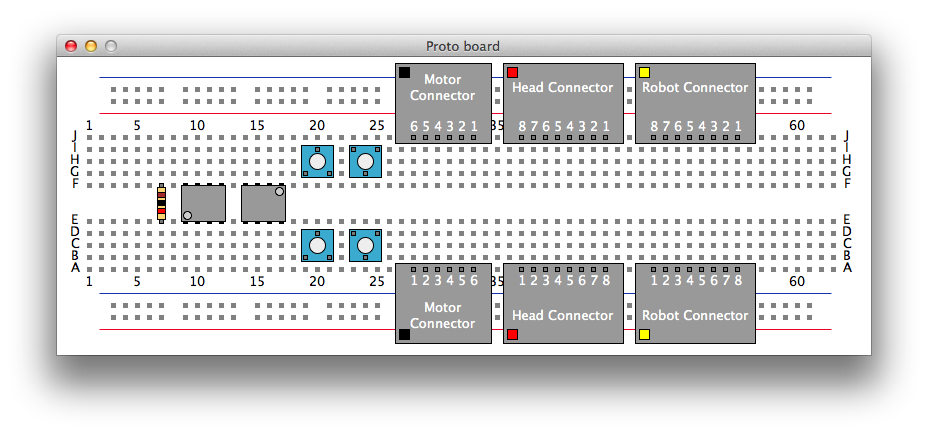
\includegraphics[width=\linewidth]{Images/piece_placement_options.png}
\caption[Acceptable circuit piece placements]{Various acceptable ways of
placing each of the circuit pieces on the protoboard.}
\label{fig:piece_placement}
\end{center}
\end{figure}

There are many ways of choosing a placement for a set of circuit pieces.
First, we must choose from a possibly large number of ways
to package together the op-amps. Section \ref{sec:justify_placement} more
precisely discusses the number of different ways of packaging op-amps.
For each possible packaging of the
op-amps, we must consider various ways of placing the pieces on the protoboard,
even with the restrictions on the ways that the pieces can be placed.

\subsubsection{Simplifications}

We reduce the number of options by only allowing placements in which no
two pieces share a $5$-column. This is not necessary in general, but the
number of pieces in the most complex 6.01 circuit is small enough that
any 6.01 circuit could likely be realized under this simplification.
Next, we specify that there must be exactly two columns on the protoboard
separating adjacent pieces, unless the pieces are both resistors, in which
case there must be exactly one column separating them. These numbers of columns
were chosen to leave enough space for wiring. Given a set of pieces to be placed
on the protoboard, these simplifications reduce the
problem of choosing a placement for the pieces to finding an \emph{order} of the
pieces together with choosing their respective vertical locations and
orientations. Figure \ref{fig:sample_placements} shows two alternative
placements for the schematic shown in Figure \ref{fig:gui_example} that both
respect the conditions put forth in the simplifications.
We consider a few alternatives to automatically finding placements respecting
these conditions.

\begin{figure}
\subfigure[Placement 1]{
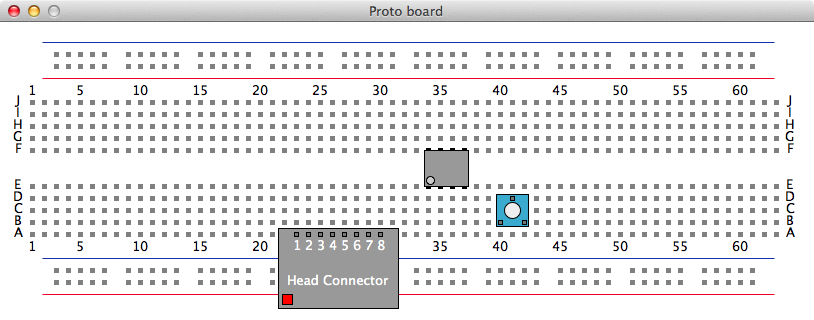
\includegraphics[width=\linewidth]{Images/sample_placement_1.png}}
\subfigure[Placement 2]{
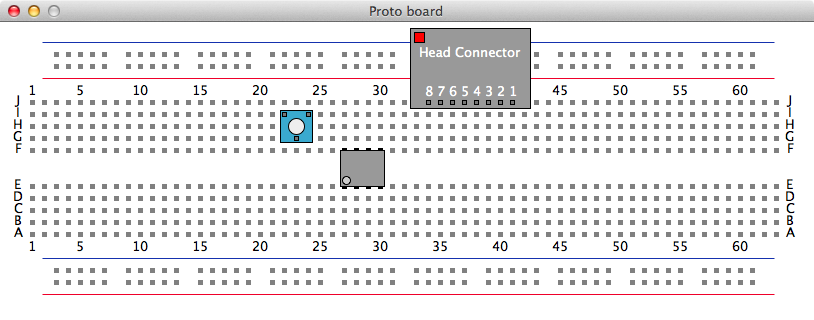
\includegraphics[width=\linewidth]{Images/sample_placement_2.png}}
\caption[Placement examples]{Two possible placements for the schematic shown in
Figure \ref{fig:gui_example}.}
\label{fig:sample_placements}
\end{figure}

\subsubsection{Random Placement}
\label{sec:random_placement}

One simple placement strategy is to choose a placement randomly.
That is, to choose
an op-amp packaging randomly; to choose an order of the pieces randomly; and to
choose the vertical locations and orientations of the pieces randomly as well.
The advantage of this
approach is that it produces a placement very quickly without requiring much
computation. On the other hand, it may place two pieces that need to be
connected to each other very far apart, which could make the wiring task more
difficult. We ought to consider alternatives that try to place the pieces so as
to require as little work as possible during the wiring step.

\subsubsection{Small Heuristic Cost}

The key idea is that if two pieces are meant to be connected together by wires,
then they should be placed close to each other on the protoboard. We can
capture this idea by assigning heuristic costs to the placements and choosing
a placement that has a small heuristic cost. To that end, there are two
heuristic cost functions we considered.

\paragraph{Distance Based Cost}
Given a circuit
schematic and a corresponding placement of the circuit pieces on the protoboard,
every pair of components in the schematic that is connected by wires indicates
a corresponding pair of
locations on the protoboard that must be connected by wires. We can
express this requirement a little bit more concisely. We must consider all
of the nodes in the circuit, and find the circuit components in the schematic
that are connected to the respective nodes. For each node in the circuit, we
get a set of locations on the protoboard that must be interconnected by wires.
The first step in devising the distance based cost function is to have a way to
estimate the cost of connecting two locations on the protoboard. A simple
cost function is the Manhattan distance between the two
locations. Since we want to produce layouts that only contain
horizontal and vertical wires (i.e. no diagonal wires), the Manhattan distance
cost is appropriate. Given this heuristic cost for connecting two locations with
wires, we can define the cost for interconnecting the locations
associated with a particular node to be the weight of the minimum spanning tree
of the locations. We can now define the cost of a placement to be the sum over
all nodes in the circuit of the cost for interconnecting the locations for each
node.

We demonstrate this cost function using the two placements shown in Figure
\ref{fig:placement_costs}. In the Figure, each placement has two connections
that must be made, the first indicated by two locations outlined by circles, and
the second
indicated by two locations outlined by rectangles. The distance based cost for
Placement 1 is $(3) + (2 + 3) = 8$ while the distance based cost for Placement 2
is $(7) + (2 + 3) = 12$. Hence, the cost function indicates that Placement 1
is a better placement of the pieces.

\paragraph{Blocking Based Cost}
The most scarce resource on the protoboard are the rows.
For a given placement, we can attempt to quantify how heavily
the rows will be used, and this quantity can be used as a placement cost.
Given a placement, we can find a set of pairs of locations on the protoboard
that need to be connected as we did above. For each $5$-column on
the protoboard, we can count the number of rows taken up by the piece that
resides in that $5$-column, if any, and the number of rows that may be taken
up in connecting the pairs of locations that must be connected. This produces
a cost for each $5$-column that indicates how heavily the rows will be used
in that $5$-column. The final heuristic cost for the placement is computed
as the sum of the squares of the costs for each of the $63 \times 2 = 126$
$5$-columns on the protoboard. We compute the sum of the \emph{squares} to
strongly penalize heavily blocked $5$-columns.

To demonstrate this cost function, let us look at the two placements in Figure
\ref{fig:placement_costs} once again. Each of the $5$-columns on both
protoboards is labeled with its cost, computed as described above.
The cost for Placement 1 is the sum of the squares of the costs for each
$5$-column, which
evaluates to $65$. The cost for Placement 2, computed similarly, is $87$. Once
again, this cost function indicates that Placement 1 is a better placement of
the pieces.

\begin{figure}[H]
\centering
\subfigure[Placement 1]{
\fbox{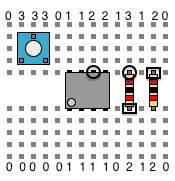
\includegraphics[width=4.5cm]{Images/placement_example_1.png}}}
\subfigure[Placement 2]{
\fbox{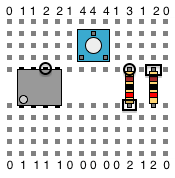
\includegraphics[width=4.5cm]{Images/placement_example_2.png}}}
\caption[Placement cost function examples]{In both placements, there are two
pairs of locations that need to be connected, denoted by either two circles or
two rectangles. Using the distance based cost function, Placement 1 has a cost of
$8$ and Placement 2 has a cost of $12$. Using the blocking based cost function,
Placement 1 has a cost of $65$ and Placement 2 has a cost of $87$. The labels
on each of the $5$-columns indicate the costs for the $5$-columns under the
blocking cost model.}
\label{fig:placement_costs}
\end{figure}

Using one of the two cost functions discussed above, we can aim to find a
placement with the minimal cost. However, this involves trying all possible
orderings of the pieces with which we are working. For example, if we are trying
to order $10$ pieces, we would need to look at $10! = 3,628,800$ possible
orderings. Note that this is in addition to
searching over all possible ways
of packaging the op-amps together. It is clear that the search for a
minimal cost placement quickly gets out of hand.
Rather than looking for an optimal placement, we aim for a placement with small
cost.

Algorithm \ref{alg:small_cost_placement} presents a polynomial-time procedure
that orders a
given list of pieces in a way that results in a small cost. The algorithm places
one of the pieces at a time, starting from an empty placement. It employs
two ideas. First, once a piece has been placed, all the pieces that are
connected to it will be placed soon after so that it is more likely that those
pieces are placed close to it. Second, we place the pieces with the most nodes
first since those are the ones that most likely have connections with many other
pieces.

The implementation of Algorithm \ref{alg:small_cost_placement} we use for the
tool may produce different placements on multiple runs. This is a side
effect of some of the data structures used to store objects -- Python sets and
dictionaries. As a result, the layout algorithm may generate different layouts
for the same circuit on different runs.

\begin{algorithm}
\KwData{A list $P$ of circuit pieces.}
\KwResult{A list $R$ of circuit pieces representing a placement.}
\BlankLine
Sort $P$ in decreasing number of nodes on the respective pieces.\\
$Q$ $\leftarrow$ empty Queue.\\
$R$ $\leftarrow$ empty List.\\
\While{$P$ is not empty}{
Pop the first piece out of $P$ and push it onto $Q$.\\
\While{$Q$ is not empty}{
$p$ $\leftarrow$ $Q$.pop().\\
Consider all vertical locations and orientations of $p$.\\
Insert $p$ at an index in $R$ that minimizes the cost of $R$.\\
\ForEach{piece $q$ in $P$ connected to $p$}{
Pop $q$ out of $P$ and push it onto $Q$.\\
}}}
\caption{Producing a circuit piece placement with small heuristic cost.}
\label{alg:small_cost_placement}
\end{algorithm}

\subsection{Part 2: Wiring}

Once the placement task is done, the next problem is wiring.
We approach this problem as a search problem and use the $A*$ Search algorithm to
solve it. In fact, the wiring step uses an infrastructure for the $A*$ Search
algorithm exactly as presented in 6.01. Hence, students in
the class may appreciate an application of something they learned
earlier in the course to produce a tool that they are using for something that
may seem completely unrelated and difficult.

\subsubsection{Using $A*$}

The $A*$ algorithm can be used to search for a path from some starting
vertex\footnote{The preferred terminology is ``a node in a graph'' but here we
will use the term ``vertex'' since we already use ``node'' to refer to nodes in
circuits.} in
a graph to some goal vertex\footnote{In fact, $A*$ guarantees an optimal path, a
path that has the minimum possible cost from the starting vertex to a goal
vertex, if we use a heuristic that is \emph{admissible}. A heuristic is said to
be admissible if it does not overestimate the actual minimal cost to a goal
vertex
for any state. Here, however, we will not worry about the admissibility of our
heuristic as our main goal is pruning out as many states as possible, while not
necessarily finding the optimal solution.}.
The algorithm works by keeping track of an agenda
of vertices to consider
in a priority queue, where the value associated with each vertex in the priority
queue is the sum of the cost to get from the start vertex to the vertex at hand
and the value of the heuristic
computed at the vertex, which is an estimate of the minimum
cost to get from the vertex to a goal vertex.
At each step, the algorithm pops
one vertex from the priority queue (the vertex with the minimum associated
value). If the vertex happens to satisfy the goal of
the search, the algorithm returns the state for that vertex as the answer to
the search
problem. Otherwise, it adds the children vertices of that vertex to the priority
queue and continues. When adding children vertices, the algorithm takes care not
to reconsider
states that it has already considered via a different path. We call the process
of popping a vertex from the priority queue and treating it as described
\emph{expanding} the vertex.
In general, when using the $A*$ algorithm, we need to design four things:

\begin{enumerate}
\item The notion of a vertex in the
search tree, the cost associated with a vertex, and how we obtain the neighbors
of a vertex,
\item The starting vertex,
\item How we identify whether a particular vertex in the search tree achieves
the goal of the search, and
\item A heuristic function that estimates the distance from a given vertex to a
goal vertex.
\end{enumerate}

\subsubsection{Vertices}
\label{sec:vertices}

Each graph vertex will represent a protoboard layout and a set of locations on
the protoboard that have yet to be connected by wires. The starting vertex will
represent a partial protoboard layout that has the circuit pieces (and possibly
some wires), as well as all the pairs of locations that must be connected by
wires to complete the layout.

We obtain the neighbors of a vertex by taking the current protoboard layout and
producing new ones in which we place exactly one new wire. We
choose the starting point of the wire to be any one of the free locations on the
protoboard that is already connected to one of the pieces, and we extend the
wires in all possible vertical and horizontal directions up to some fixed wire
length. For a location on a rail row, we only extend vertical wires that reach
to either another rail row, or any location in either of the $5$-columns that
are vertically aligned.
For a location on a $5$-column, we extend horizontal wires that reach other
$5$-columns (in both directions), as well as
vertical wires that reach the rail rows or any location on the other
$5$-column that is vertically aligned.
Note that the process needs
to take great care when placing new wires in order not to short, or directly
connect, two different nodes.

The way we define the cost of a vertex, i.e. the cost of getting from the
starting vertex to a vertex of interest, depends on our definition of a good
protoboard layout. In general, we want to penalize having
long wires, many wires, or crossing wires. In our implementation, while we have
a large penalty for two crossing wires of opposite orientations (i.e. vertical
and horizontal), we do not allow occlusions as
they are particularly difficult to physically build and debug.
In addition, we favor making a desired interconnection between locations
on the protoboard. That is, if placing one wire results in a layout in which
one of the pairs of locations that needs to be connected becomes connected, then
the cost of that child vertex should reflect that fact. More precisely, in an
attempt to connect locations $\text{loc}_1$ and $\text{loc}_2$, a wire placed extending from
$\text{loc}_1'$ to $\text{loc}_{\text{mid}}$, where $\text{loc}_1'$ is a
location connected (internally or by wires) to
$\text{loc}_1$ and
$\text{loc}_{\text{mid}}$ is a free location, the additional cost
incurred by adding the wire is computed as:
\begin{table}[H]
\centering
\begin{tabular}{ccllr}
-100 &$\times$ & ($\text{loc}_1$ and $\text{loc}_2$ now connected) &+ &($1$)\\
1 &$\times$ & ($d$($\text{loc}_1'$, $\text{loc}_{\text{mid}}$) + $d$($\text{loc}_{\text{mid}}$, $\text{loc}_2$) - $d$($\text{loc}_1$, $\text{loc}_2$)) &+ &($2$)\\
100 &$\times$ & (number of crossed wires) &+ &($3$)\\
10, & & & &($4$)
\end{tabular}
\end{table}
\noindent where $d$($\text{loc}_i$, $\text{loc}_j$) is the Manhattan distance
on the protoboard from $\text{loc}_i$ to $\text{loc}_j$.
Line ($1$) decreases the cost by $100$ if a new connection is
made. Line ($2$) penalizes long wires, taking into account how much closer (or
farther) the new wire gets us to connecting locations $\text{loc}_1$ and
$\text{loc}_2$.
Line ($3$) adds a cost of $100$ for each new pair
of crossing wires. Line ($4$) adds $10$ to the total cost to penalize having
too many wires. We produced this cost metric experimentally by thoroughly
testing various ideas on a selected set of circuit schematics.

An important consideration we need to make is how to organize the
search. Recall that we have a set of nodes in the circuit of interest, and for
each node we have a set of locations that need to be interconnected.
We considered the following six different strategies to carry out the search:

\begin{enumerate}
\item All pairs: Collect all pairs of protoboard locations that need to be
connected for all nodes in the circuit, and have the starting vertex represent
this set of pairs of locations. In this strategy, we run exactly $1$ search to
solve the problem.
\item Per-node (increasing): Treat each node individually. That is, iteratively
connect the locations for each of the nodes until there are no more disconnected
nodes in the circuit. In this strategy, we run a number of searches equal to the
number of nodes in the circuit. Order the searches in
\emph{increasing} order of the number of locations per node, breaking ties
arbitrarily.
\item Per-node (decreasing): Similar to per-node (increasing), but order the
searches in \emph{decreasing} order of the number of locations per node.
\item Per-pair (increasing): Treat each pair of locations that needs to be
connected individually. That is, iteratively connect pairs of locations that need
to be connected until there are no more disconnected pairs.
In this strategy, we run a number of searches equal to the number of pairs of
locations that must be connected. Order the searches in \emph{increasing} order
of the Manhattan distance between the pairs of locations, breaking ties
arbitrarily.
\item Per-pair (decreasing): Similar to per-pair (increasing), but order the
searches in \emph{decreasing} order of Manhattan distance between the pairs of
locations.
\item Straight: As a back-up alternative, we consider using one (possibly
diagonal) wire to connect
each of the pairs of locations that must be connected. This approach requires no
search and does not take layout quality into consideration.
\end{enumerate}

The strategy we choose among these six
has a significant effect on the outcome of the wiring step.
We discuss the differences in detail in Chapter \ref{ch:results}.

\subsubsection{Goal test}

We say that a given vertex is a goal vertex by verifying that its
representation indicates no further pairs of locations to connect.

\subsubsection{Search heuristic}

In $A*$ search, choosing the right heuristic can often make the search much more
efficient. Given a
vertex, we can estimate its distance from a goal as follows. For each pair of
locations $(\text{loc}_1, \text{loc}_2)$ that needs to be connected, we could
consider the pair's distance from a
goal to be the smallest Manhattan distance between any location connected to
$\text{loc}_1$ and any other location connected to $\text{loc}_2$.
To compute the heuristic
cost of a vertex, we simply sum this value over all pairs of locations
that need to be connected. In Chapter \ref{ch:results}, we compare the
performance of $A*$ with this heuristic versus carrying out Best First Search
with this heuristic. In Best First Search, as opposed to in $A*$, vertices are
considered in order of increasing heuristic value, without consideration for
the cost incurred on the path from the starting vertex.

\subsubsection{Limiting the number of expanded vertices}

In the implementation of $A*$ discussed so far, the algorithm
terminates if we either find a solution, or we
exhaust the search space without finding a solution. In our search problem, the
search space size is very big (Section \ref{sec:search_space_size} discusses
the search space size
in more detail), so this implementation of $A*$ may sometimes run out
of memory before returning an answer.
To mitigate this problem, we introduce a limit to
the number of vertices the algorithm expands before giving up. That is, if the
algorithm expands a certain fixed number of vertices and still has not found an
answer, it gives up. We set this limit to $300$ vertices.
In Chapter \ref{ch:results} we provide data that motivates this choice and
describes the effect of this choice on each of the alternatives discussed above.

\subsection{Combining the Methods}
\label{sec:combined_alg}

With the methods discussed so far, we aimed to completely solve the layout problem
with one placement method and one wiring method. However, as we will soon see,
such an algorithm is bound to fail on some set of schematics. When we ultimately
put the final algorithm in front of students, we would like to avoid failure.
The algorithm should be able to generate a layout for any schematic.
Generating a layout
with a few diagonal or crossing wires is better than silently failing and leaving
the student empty handed. Here, we discuss how we combine the methods
described so far into one layout algorithm. The motivation for this combination
is discussed in Chapter \ref{ch:discussion}, based on the data we obtained
for the alternatives described thus far.
Algorithm \ref{alg:combined} presents the
combined algorithm.

\begin{algorithm}
\KwData{A circuit schematic $C$.}
\KwResult{A protoboard layout corresponding to $C$.}
\BlankLine
\ForEach{Placement cost metric $M$ in (DISTANCE, BLOCKING)}{
$P$ $\leftarrow$ Placement for $C$ by using cost metric $M$.\\
Connect the top and bottom rails on $P$.\\
\ForEach{Order $O$ in (INCREASING, DECREASING)}{
$pairs$ $\leftarrow$ Pairs of location on $P$ to connect given schematic $C$ and connection order $O$.\\
\ForEach{$(\text{loc}_1, \text{loc}_2)$ in $pairs$}{
Attempt to connect $loc_1$ and $loc_2$ on $P$.\\
If successful, update $P$ accordingly and then post-process $P$.\\
If not, record that the pair $(loc_1, loc_2)$ was not successfully connected.\\
}
If all pairs are successfully connected, return $P$.\\
}}
Pick unfinished layout with fewest and most compact disconnected pairs.\\
Connect remaining pairs with shortest possible wires (possibly diagonal).\\
Post-process and return resulting layout.\\
\caption{Layout algorithm obtained by combining multiple alternatives.}
\label{alg:combined}
\end{algorithm}

Algorithm \ref{alg:combined} uses the per-pair wiring scheme discussed above,
and works by attempting to solve the problem in four different ways:
two different ways of doing placement together with two different orders of
wiring pairs. If any one of the four trials
succeeds, the algorithm immediately returns the corresponding layout. If all
four trials fail, on the other hand, the algorithm picks one of the four
unfinished layouts that has
the fewest disconnected pairs of locations (breaking ties by considering
wire lengths and
wire-piece crossings) and completes the solution by connecting the disconnected
pairs using one wire per pair chosen to maximize goodness among
all equivalent pairs of locations.
This last step makes
it highly unlikely that the algorithm will ever fail;
the only way for the algorithm to fail is for there to be two nodes on the
protoboard that need to be
connected where all of the protoboard locations for at least one of the nodes are
occupied, which is highly unlikely. This high success rate comes at the
cost of placing wires that may significantly reduce the goodness of the layout.

The algorithm starts out by connecting the top and bottom rail
rows of the protoboard
so that all rail rows are used to connect to power and ground, and no other
nodes. This is a restriction that makes it easier to debug and amend the
resulting layout. Without this restriction, some rail rows might be used for
nodes that are neither power nor ground, and this may confuse some students.

The algorithm also has a post-processing step that attempts to to improve the
layout. The post-processing step makes three types of simple changes to the
layout:
\begin{itemize}
\item We throw away any superfluous wires that do not serve to connect
two parts of the circuit. Superfluous wires may be added to the layout
in the search done by the wiring step, though very rarely.
\item We truncate
long vertical wires into an equivalent set of smaller wires. For example, a wire
going from one of the top rails to one of the bottom rails can be replaced by
three smaller wires making the same connection. This change frees up rows for
subsequent connections.
\item If shifting a horizontal wire up or down
results in a layout with fewer crossing wires, we make that change.
\end{itemize}

The last important aspect of this final algorithm not explicitly stated in
Algorithm \ref{alg:combined} is that the algorithm that will be put
in front of students will only be allowed to use wires of a select few lengths.
The kits that students work with do not come with wires of all lengths,
so we force the wiring step to use wires of only those allowed lengths. We also
avoid using length-$1$ wires because they are difficult to insert and
remove from physical protoboards and are also difficult to see.

\subsection{Evaluation}

Here we present how we evaluated our solution to the automatic layout problem
to test how well it would serve students in 6.01.
We ran the layout algorithm on numerous schematics and
analyzed its performance on generating layouts from those schematics.
As manually generating
numerous test schematics is tedious and time-consuming, we devised a method
to randomly generate thousands of test schematics. As the tool targets 6.01 labs,
we tried to design the randomly generated schematics so that the range of
complexity of these schematics mimics the range of complexity of circuits that
students may build in 6.01.

The random schematic generation goes as follows. We created $6$ basic parts
of schematics. These $6$ bases are:
\begin{itemize}
\item Three resistors arranged in a T-shaped configuration.
\item Two resistors in series connected to a follower op-amp configuration.
\item A pot connected to a follower op-amp configuration.
\item A motor.
\item A robot head.
\item A robot.
\end{itemize}
These bases are depicted in Figure
\ref{fig:random_gen_bases}. They cover all of the components that may be
necessary in a 6.01 circuit. Each base offers at least $3$ points of
connection with other bases. The random generation algorithm takes all
possible combinations of up to
$6$ bases, allowing for repetition of bases with some restrictions.
The robot head and robot bases can appear at most once as there is
no need for more than one of each of these in 6.01 labs. The pot and follower
op-amp base can appear at most twice as we never need more than two pots in 6.01
circuits. The motor base can also appear at most twice as we never need more
than two motors per circuit in 6.01 labs. The other two bases, T-resistor
configuration and two resistors in series together with a follower op-amp, can be
repeated up to 6 times. For a given combination of bases, we generate a
set of schematics in which we randomly make connections between the
bases. Figure \ref{fig:example_random_schematic} presents a sample randomly
generated schematic.

\begin{figure}[H]
\begin{center}
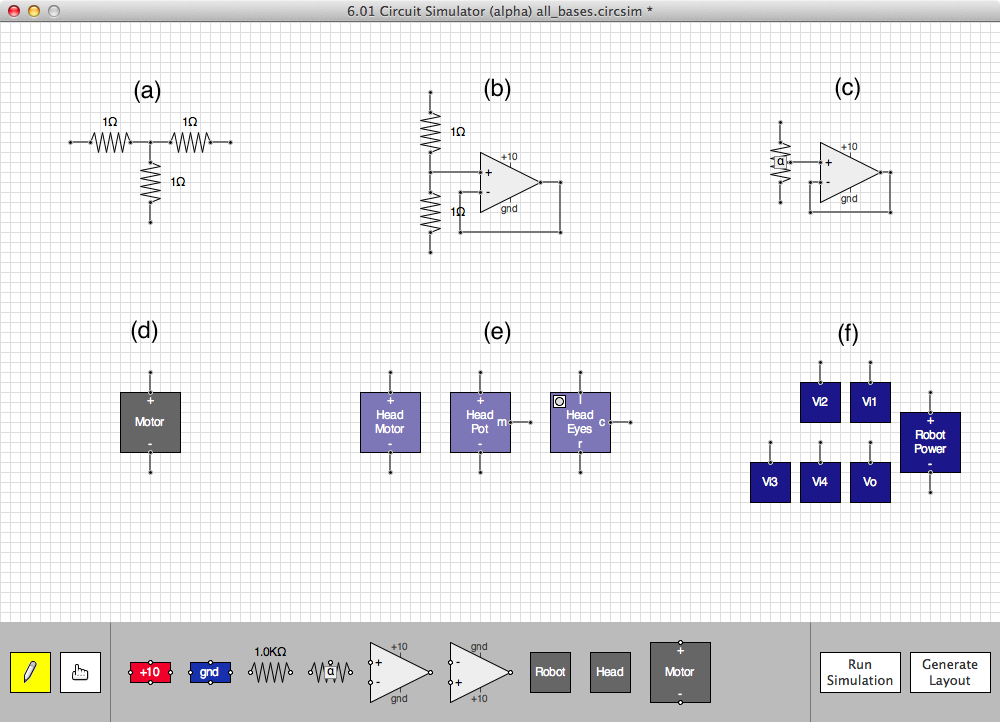
\includegraphics[width=\textwidth]{Images/auto_generation_bases.png}
\caption[Random schematic generation bases]{Bases for the random schematic
generation scheme:
(a) three resistors arranged in a T-shaped configuration;
(b) two resistors in series connected to a follower op-amp configuration;
(c) pot connected to a follower op-amp configuration;
(d) motor;
(e) robot head; and
(f) robot.}
\label{fig:random_gen_bases}
\end{center}
\end{figure}

\begin{figure}[H]
\begin{center}
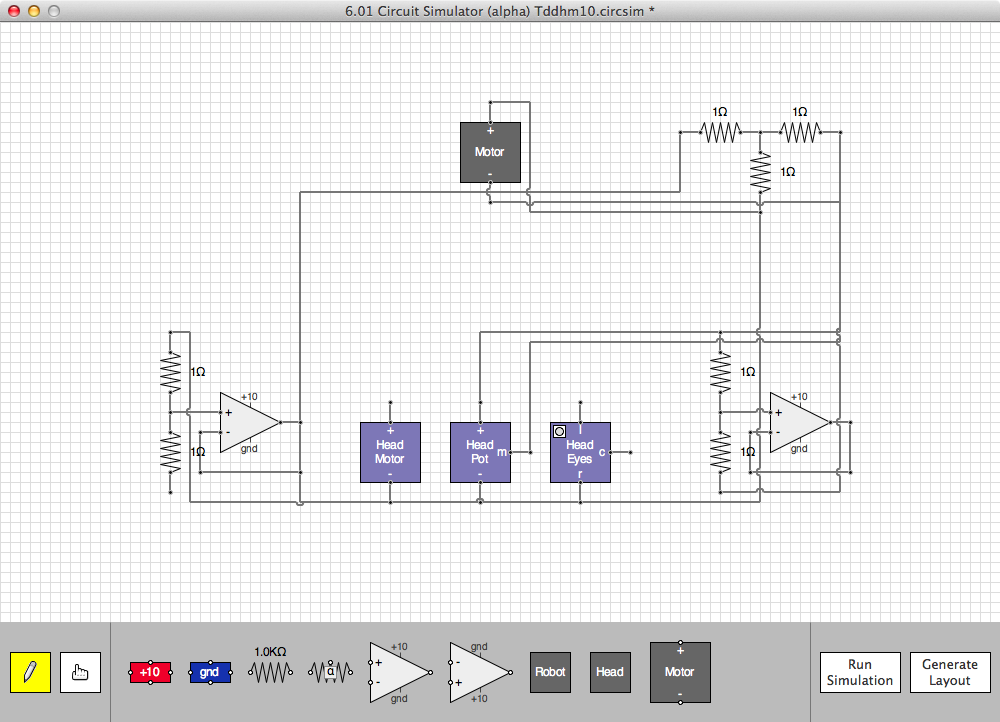
\includegraphics[width=\textwidth]{Images/auto_generation_example.png}
\caption[Sample randomly generated schematic]{Sample randomly generated
schematic.}
\label{fig:example_random_schematic}
\end{center}
\end{figure}

Our scheme produces a total of $4425$ test schematics.
When testing a particular algorithm on these test
schematics, we run the algorithm on each test schematic $10$ times. Chapter
\ref{ch:results} presents the data collected in this manner and compares the
various alternatives discussed in this chapter.

An important question we must answer is how we quantify the goodness (or badness)
of a particular layout. Our approach takes a weighted sum of a particular set of
features of a given layout. We define the badness of a layout to be:
\begin{table}[H]
\centering
\begin{tabular}{ccll}
1 &$\times$ &(number of wires) &+ \\
2 &$\times$ &(total wire length) &+ \\
10 &$\times$ &(number of wire crosses) &+ \\
10 &$\times$ &(number of diagonal wires) &+ \\
50 &$\times$ &(number of wire-piece crossings) &+ \\
500 &$\times$ &(number of wire occlusions).
\end{tabular}
\end{table}
We use this metric to decide which of a given set of alternative
layout generation strategies tends to produce better layouts.
The weights in the metric were chosen to reflect how
bad each of the features is relative to the others. This choice of weights,
therefore, reflects the following reasonable set of statements. Recall that our
goal is to produce layouts that are easy to build, easy to debug, and
aesthetically pleasing.
\begin{itemize}
\item Having an additional wire is about as bad as increasing the total wire
length on the protoboard by $2$.
\item Having two wires that cross is about as bad as increasing the total
wire length on the protoboard by $5$.
\item A diagonal wire is about as bad as a pair of wires that cross.
\item Having a wire that crosses a circuit piece is about as bad as having $10$
pairs of wires that cross.
\item Having a wire occlusion is about as bad as having $10$ wires that cross
circuit pieces.
\end{itemize}

Note well that the badness metric described here is different from the cost
metric used in the wiring search as described in Section \ref{sec:vertices}.
This badness metric is used to evaluate layouts produced by the algorithm,
which may use $A*$ search in which the costs of vertices are computed, not using
this badness cost metric, but the cost metric described in Section
\ref{sec:vertices}.
